	\begin{comment}
	  \part*{INTRO "`respiratory system"'}
		  \emph{Materials needed:}
			  \begin{itemize}
			   \item hydra - the plastic model
			   \item earthworm - the plastic model
			   \item insect - model or specimen
			   \item Fish - the plastic model
			   \item Frog - the plastic model (??)
			   \item human - the skeleton
			       \item print the following page as an OP transparency
% 	               \item container and water to illustrate the vital capacity
	               \item transparency with gas exchange
	               \item flow meter
			  \end{itemize}



	  \clearpage

	  \clearpage
	  \begin{Large}
	  You all know:
		   \begin{itemize}
	               \item cell respiration takes place in the mitochondriae
	               \item cell respiration requires  \ce{O2} according to  \ce{C6H12O6 + 6 O2 ~ ->~ 6 H2O + 6 CO2}
	             \end{itemize}

	             \vspace{1cm}
	\rule{16cm}{1pt}
	             \vspace{1cm}

	What do you know about \emph{respiration}, gas exchange and transport of oxygen?

			\begin{enumerate}[label=\textit{(\arabic*)},leftmargin=0em,series=zaehler]
			      \item Check the models of different organisms on display: how can oxygen travel from the air to any single cell in those organisms?

			      \item Check the skeleton and compare with your own rip cage: how is air taken into your body? How can you illustrate your answer with a body activity?

			      \item Imagine your lungs: how should they be constructed in order to efficiently take up oxygen from the air?

			      \item You know there is \emph{hemoglobin} in every erythrocyte - how does this protein help to transport oxygen?
			\end{enumerate}


	\end{Large}   \clearpage \addtocounter{page}{-2}
	\end{comment}



\section{The respiratory system}\label{sec:RespiratorySystem}
\subsection{Routes of oxygen}
According to the summarized cell respiration, every cell of an \emph{aerobic} organism requires oxygen (\ce{O2}). Complete the equation:  \ce{C6H12O6} + \gap{\ce{ 6 O2 ~ ->~ 6 H2O + 6 CO2}}

		\begin{mdframed}[style=exampledefault, userdefinedwidth=12cm,frametitle={Starr, chapter 35.1 and 35.2}\label{mat:BEISPIELMATERIAL}]
		Depending on the level of organisation, there are different routes and different organs to deliver oxygen from the outside, the environment, to every single cell of an organism.
		\end{mdframed}

	 \begin{enumerate}[itemsep=1.5em, leftmargin=*]
	\item  Read \ding{229} 35.1 and 35.2 and fill in the following table \ref{tab:O2Transport}!
	\end{enumerate}

	\begin{table}[!htbp]
	\setlength{\extrarowheight}{6pt}
	\captionof{table}[oxygen pathways]{How oxygen reaches the cells}
	  \vspace{12pt}  \hspace{0cm}
	    \begin{tabularx}{16cm}[]{p{3cm} p{4cm} X} %
	\toprule
	Organism & route of  \ce{O2}  &  \ce{O2}-uptake system: short summary  \\\midrule
	 Paramecium (1 cell) &  across the cell membrane & solely by diffusion; no special structures (\textit{... its a single celled organism!...}) \\[1.1cm]
	 Hydra (many cells) & \gap{ across cell membranes} & \gap{diffusion} \\[1.1cm]
	 Earth worm &  \gap{skin cell $\rightarrow$~ blood vessels $\rightarrow$~ body cells } & \gap{diffusion, blood flow} \\[1.1cm]
	 Insect &  \gap{trachea, membranes of trachea and cells} & \gap{air movement, diffusion} \\[1.1cm]
	 Fish &  \gap{gills, membrane of gill, blood, cell membrane} & \gap{diffusion, blood flow} \\[1.1cm]
	 Frog &  \gap{skin $\rightarrow$~ blood, primitive lung $\rightarrow$~ blood} & \gap{diffusion, blood flow} \\[1.1cm]
	 Human &  \gap{lungs $\rightarrow$~ blood} & \gap{diffusion, blood flow} \\[1.1cm]
	\bottomrule
	\end{tabularx}%
	  \label{tab:O2Transport}%
	\end{table}%
%


\subsection{The human respiratory system}
The overall goal of the respiratory system in mammals is the  maximisation of the respiratory surface, enabling the organism to efficiently take up oxygen.

		\begin{mdframed}[style=exampledefault, userdefinedwidth=12cm,frametitle={Starr, chapter 35.4}\label{mat:BEISPIELMATERIAL}]
			This is an integral part of our syllabus: read and revise this topic with your textbook.
		\end{mdframed}

\vspace{6cm}



\subsection{The respiratory cycle}
The main principle of in- and expiration in animals that have a rip cage is v\gap{entilation}

		\begin{mdframed}[style=exampledefault, userdefinedwidth=12cm,frametitle={Starr, chapter 35.5}\label{mat:BEISPIELMATERIAL}]
			Only the first section \textit{``The respiratory cycle''} applies here. (See chapter \titelref{sec:HomeostaticControl}, page \pageref{sec:HomeostaticControl} for \textit{``control of breathing''})
		\end{mdframed}

	\begin{enumerate}[resume, leftmargin=*]
	\item  Comment the following figure (\ref{fig:RespiratoryCycle}) according the instructions given in \ding{229} Starr
	\end{enumerate}



		 		\begin{figure}[htp]
		  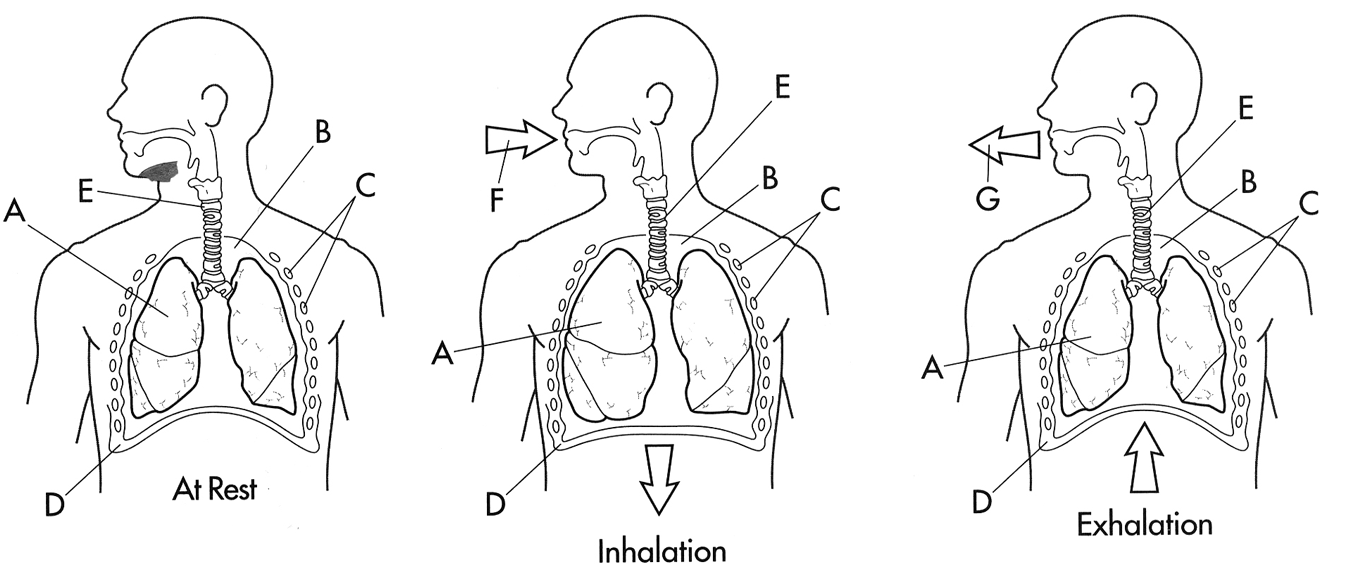
\includegraphics[width=12cm]{../images/BiolColBook-265-fig1.png}
		  \caption[Respiratory cycle; Biology Coloring Book p. 265]{Respiratory cycle of a human}
		  \label{fig:RespiratoryCycle}
% 		\setfloatalignment{b}
		\end{figure}


\clearpage
\subsection{Gas exchange and transport}

	\marginnote{\caution[t][BrickRed][hint!]{The process of \textbf{diffusion} drives the exchange of gases in your body, of oxygen in and carbon dioxide out of your body cells.}}

		\begin{mdframed}[style=exampledefault, userdefinedwidth=11.5cm,frametitle={Starr chapter 35.6}\label{mat:BEISPIELMATERIAL}]
			The coloured figures nicely allow for a clear understanding of the \textit{``air bags''}, the \emph{alveoli} and the distributions of  \ce{O2} on the one hand and  \ce{CO2} on the other hand. Carefully read this section.
		\end{mdframed}

	\begin{enumerate}[resume, leftmargin=*]
	\item  Define the term \emph{partial pressure of a gas} - see \ding{229} p.622:
	\Loesung{The \textbf{partial pressure} of a gas is its contribution to the pressure of a mixture of gases. In fresh air these are approximately 78\%  \ce{N2}, 21\%  \ce{O2}, 1\%  (\ce{Ar}, \ce{Kr},\ce{Xe}), 0.04\%  \ce{CO2} }{1.7cm}

	\item Read \ding{229} Starr 35.6, section \emph{oxygen transport} and explain the role of the erythrocytes (\textit{=red blood cells}) for the transport of oxygen!
		\Loesung{Oxygen binds to hemoglobin, or even more precisely to the \emph{heme} group, the iron containing part of hemoglobin. One, two, three or four  \ce{O2} molecules may be attracted by hemoglobin.}{1.7cm}

	\item Carefully study figure \ref{fig:O2andCO2Ery} and explain the role of the erythrocytes for the transport of carbon dioxide!
		\Loesung{Carbon dioxide gas, the  \ce{CO2} enters the erythrocyte. Only a small portion binds to hemoglobin. Most of the  \ce{CO2} gas is being converted into \textit{''soluble carbon dioxide''}, the  \ce{HCO3-} anion. This substance is highly water soluble, exits the erythrocyte and is being transported in the blood plasma.
		}{1.7cm}
	\end{enumerate}


% 			\begin{figure}[htp]
% 		  \includegraphics[width=1\textwidth,angle=0]{../images/Russel-Dynamic_p1036-1_v2.png}
% 		  \caption[Processes of O2 and CO2 exchange, source: Russel, Dynamic Science, p 1036]{Transport of  \ce{CO2}; from (A) body tissues (B) to alveolar air.}
% 	  \label{fig:O2andCO2Ery}
% 		%\setfloatalignment{b}
% 		\end{figure}


		\vfill
		\hspace{-2cm}
% 		\hspace{-4cm}
	\begin{minipage}[htbp]{18cm}
		 \includegraphics[width=1\textwidth,angle=0]{../images/Russel-Dynamic_p1036-1_v2.png}
		  \captionof{figure}[Processes of O2 and CO2 exchange, source: Russel, Dynamic Science, p 1036]{Transport of  \ce{CO2}; from (A) body tissues (B) to alveolar air.}
	  \label{fig:O2andCO2Ery}
	\end{minipage}
	\vfill


\clearpage
\subsection{Myoglobin, Hemoglobin,  \ce{O2}-dissociation curves}
Myoglobin consists of one polypeptide chain and one hem group.
Myoglobin binds  \ce{O2} in the muscle. Myoglobin makes muscles red.
Hemoglobin consists of four polypeptide chains and four hem groups.
Hemoglobin binds  \ce{O2} in the blood. Hemoglobin makes blood red.


% 	\marginline{
% 		 \includegraphics[width=4.6cm]{../images/PhysiolMalatl_053-4-_Atmung-i.png}
% 		 \captionof{figure}[Hemoglobin molecule, scheme; Malatlas Physiol p.53]{Schematic view of a hemoglobin molecule}
% 	         \label{fig:HemoglobinScheme} }

The hemoglobin molecule is shown in \ding{229} Starr  Figure 35.15: four subgroups can be identified, two in blue and two in green and four hem groups, shown in red. Each protein chain forms a pocket big enough to store one molecule of  \ce{O2}, thus the four protein chains can bind four  \ce{O2} molecules.
%
% 	\marginnote{
% 		 \includegraphics[width=5cm]{../images/PhysiolMalatl_053_v2.png}
% 		 \captionof{figure}[hemoglobin, T- and R-form, from Malatlas Phyisol]{Tense, \textbf{T}-form and relaxed, \textbf{R}-form of hemoglobin. }
% 	         \label{fig:HemoglobinCooperation} }

 Hemoglobin is found in two different states - the oxygenated (found in "`oxy blood"') and the deoxygenated (present in "`deoxy"' blood) condition. Biochemically this is well understood:

 In \emph{deoxy-hb} all four sub units are very close together and form a tight block due to ionic forces (\textit{like what keeps salt molecules together}). This form is called \emph{tight} and abbreviated as \textbf{T}-form.

 In \emph{oxy-hb} one or more of the sub units carry a  \ce{O2}-molecule. As soon as the first  \ce{O2}-molecule binds to the hemoglobin, the four subunits move apart a little bit, making it easier for the second, third and fourth  \ce{O2}-molecule to bind at the remaining sub units. Under this circumstance the hemoglobin molecule seems to be \emph{relaxed}, therefore it is called \textbf{R-}form (see figure \ref{fig:HemoglobinCooperation}). Due to this irregularity in  \ce{O2}-affinity, the resulting   \ce{O2}-dissociation curve is \textbf{S-shaped} instead of being linear (see figure \ref{fig:HbAffinitaetskurve}).


			\begin{figure}[htp]
		  \includegraphics[width=9cm]{../images/PhysiolMalatl_054-1_Atmung-i_v1.jpg}
		  \caption[Hb Affinitätskurve aus Malatlas Physiol]{Course of the normal  \ce{O2}-dissociation curve of hemoglobin.}
		\label{fig:HbAffinitaetskurve}
		%\setfloatalignment{b}
		\end{figure}


	\clearpage
	\begin{enumerate}[resume, leftmargin=*]
	\item  Figures \ref{fig:HemDissCurveLung} and \ref{fig:HemDissCurveTissue} are highly similar to figure \ref{fig:HbAffinitaetskurve} - but in greater details. Now, explain the shift of the dissociation curve in figure \ref{fig:HemDissCurveTissue} that comes along with the change in pH from 7.4 to 7.2!\\
		 \Loesung{ ... it's what the figure legend reads ... }{1.7cm}

	 \item Read again figure \ref{fig:O2andCO2Ery} and explain why the blood pH falls from 7.4 at the beginning of the systemic capillaries to pH 7.2 at the start of the  systemic veins (see  \ding{229} Starr figure 35.14 for systemic capillaries and veins).\\
		 \Loesung{Active cells give off  \ce{CO2} which reacts with water to  \ce{HCO3-} and  \ce{H+}. The  \ce{H+} is a so called ``acid particle'' - the more there is, the lower the pH reads. Summary: At the end of the capillaries there is more  \ce{H+} due to  \ce{CO2} and thus the pH is lower than at the beginning of the capillaries. }{1.7cm}
	\end{enumerate}


	\enlargethispage{2cm}
				\begin{figure}[htp]
		  \includegraphics[width=7.5cm]{../images/Russel-Dynamic_p1035-1-A_v2.png}
		  \caption[VERWEIS]{ Hemoglobin-O2 dissociation curve in the \textbf{lungs}.}
		  \label{fig:HemDissCurveLung}
		%\setfloatalignment{b}
		\end{figure}

				\marginnote[-1cm]{\caution[c][BrickRed][info]{The unit \emph{Torr} defines the length of a mercury column in a tube (= \emph{mm HG}). This unit is named after E. Torricelli who discovered the barometer. Torr is mostly used in medicine because its values are easy to remember - compare the blood pressure values, being around ``\textit{80 over 120}`` for the diastolic and systolic pressures respectively.
		\includegraphics[width=4cm]{../images/NSRW_Torricelli's_experiment_v1.jpg}
		\textit{A tube, one meter long, sealed at the top, is filled with mercury, and set vertically into a basin of mercury. The column of mercury falls to about 760 mm (76 cm). The column's height fluctuats with changing atmospheric pressure - this is a simple barometer. (from: wikipedia)}
		}}

						\begin{figure}[htp]
		  \includegraphics[width=7.5cm]{../images/Russel-Dynamic_p1035-1-B_v2.png}
		  \caption[VERWEIS]{ Hemoglobin-O2 dissociation curve in the \textbf{body tissue}.}
		  \label{fig:HemDissCurveTissue}
		%\setfloatalignment{b}
		\end{figure}


\marginnote{\caution[c][BrickRed][hint!]{The shift of the  \ce{O2}-dissociation curve due to changes in pH is called the \textbf{Bohr effect}}}

%
% A close look at figure \ref{fig:O2andCO2Ery} reveals the release of one  \ce{H+} for the production of each  \ce{HCO3-} from  \ce{CO2 + H2O} and an arrow bringing this  \ce{H+} to \textit{Hemoglobin}. There is a close link of this chemical process to the  \ce{O2}-dissociation curve of hemoglobin:
% \begin{itemize}
%  \item each  \ce{H+} forms in water a  \ce{H3O+}
%  \item every  \ce{H3O+} lowers the pH, low pH is "`acidic"'
%  \item in the body tissue the pH \gap{sinks} due to \gap{CO2} given off from the tissue
%  \item in the lungs the pH \gap{rises} due to \gap{CO2} taken away by the lungs
%  \item the lower the pH, the \gap{lower} the affinity of hemoglobin for  \gap{\ce{O2}}
%  \item the higher the pH, the \gap{higher} the affinity of hemoglobin for \gap{\ce{O2}}
% \end{itemize}


	 \areaset[0cm]{14cm}{28cm}   % = default; kann geändert werden


\begin{enumerate}[itemsep=1.5em, leftmargin=*]
\item  In addition to the number of  \ce{O2}-molecules bound to Hb and the pH value, a third factor controls the affinity of hemoglobin for  \ce{O2}: the chemical substance di-phospho-glycerol (DPG). This is best seen figure \ref{fig:HbRechtsverschiebung}: the more to the left a curve lies, the lower the concentration of DPG. The \textit{pregnant mom} depicts the  \ce{O2}-dissociation curve of a mother's blood (= an adult body). The \textit{baby} depicts the  \ce{O2}-dissociation curve of a fetus' blood inside a mother's whomb. Now explain the effect of the different concentrations of DPG present in the fetal hemoglobin (Hb\textsubscript{f}) compared to DPG present in the adult hemoglobin (Hb\textsubscript{a})!
	\Loesung{\\ The foetus' haemoglobin has a higher affinity to oxygen than mother's haemoglobin. This allows the transfer of oxygen from the mother's to the foetus' blood. Without this adaptation, the foetus would die due to a lack of oxygen.}{2.5cm}
\end{enumerate}


		\begin{figure}[htp]
		  \includegraphics[width=7.5cm]{../images/PhysiolMalatl_054-3_Atmung-i.png}
		  \caption[Hb Rechtsverschiebung, aus Malatlas Physiol]{ Effect of acids ( \ce{H+}),  \ce{CO2} oder Diphosphoglycerol (DPG) on the  \ce{O2}-affinity of hemoglobin (Hb) }
		 \label{fig:HbRechtsverschiebung}
		%\setfloatalignment{b}
		\end{figure}

\enlargethispage{2cm}
\begin{enumerate}[resume, leftmargin=*]
\item  Discuss now the  \ce{O2}-dissociation curve of \textbf{Myoglobin} in regard to the amount of DPG present, and in regard to its role as a  \ce{O2}-acceptor inside the muscle.
\Loesung{ \\ Myoglobin's higher affinity for oxygen allows for the oxygen transfer from hemoglobin to muscle.}{0.85cm}

\end{enumerate}


		\begin{figure}[htp]
		  \includegraphics[width=7.5cm]{../images/PhysiolMalatl_054-2_Atmung-i.png}
		  \caption[Myoglobin vs Hämoglobin aus Malatlas Physiol]{ Oyxgen is transferred from Hemoglobin (Hb) in the blood stream to Myoglobin (Mb) in the muscle. Explain the different shapes of these two dissociation curves!}
		\label{fig:HbUebergabeMb}
		%\setfloatalignment{b}
		\end{figure}


% 				\piccaptionoutside
% 		%\setcapmargin*[-2cm ]{0cm }
% 		\piccaption[oxygen debt after exercising; from Kent biology]{\label{fig:OxygenDebt} The effect of exercising on the oxygen uptake of your body - explain the debt of oxygen at the end of the exercise!}
% 		\parpic[r]{\includegraphics[width=12cm]{../images/Kent_p130-Fig2_oxygen-debt.jpg}}
% 		\picskip{0}
% 		%\setcapmargin*[0cm ]{0cm }
%

% 	 \areaset[0cm]{11.5cm}{27.4cm}   % = default; kann geändert werden
